\selectlanguage{ngerman}
\section{Technische Umsetzung}\label{ch:Umsetzung}
Das im Rahmen dieser Arbeit entwickelte System besteht aus drei Teil-Systemen: dem Sensor, dem Server und der App.
Dabei wird unter dem Sensor System der Teil angesehen, welcher eine klassische Detektion ersetzen kann.
Im konkreten Fall besteht dieser Teil aus einem Raspberry Pi 3 und einer Pi Kamera v2.1.
Der Server stellt die das Bindeglied der Kommunikation zwischen Sensor und App dar.
Für den Nutzer werden die erfassten Daten in der App dargestellt die vom Server gesendet werden.
Die gesamte Architektur ist in Abbildung~\ref{fig:Architektur} dargestellt.

\begin{figure}[h]
    \myImagePos{}
    \includesvg[inkscapelatex=false,width=\myImageWidth]{Bilder/Architektur_gesamt_2.svg}
    \caption[Schematische Darstellung der System-Architektur]{Schematische Darstellung der System-Architektur mit ihren einzelnen Systemen (blau), den an diesen angebundenen Komponenten (hellblau) und den zur Kommunikation verwendeten Protokollen (grün). (Quelle: eigene Darstellung)}
    \label{fig:Architektur}
\end{figure}

Im Folgenden wird jeweils auf die Umsetzung der einzelnen Teil-Systeme eingegangen.

\selectlanguage{ngerman}
\subsection{Sensor}\label{ch:Umsetzung_Sensor}
% - Objekterkennung auf Frames: vortrainierte Modelle
% - Schwierigkeit: Nicht nur Erkennung einzelner Objekte nötig, sondern Erkennung des Rein- und Rausfahrens der Autos
%     --> zwei Implementierungen, Verweis auf Tests

Die Komponente, welche erkennt, wie viele Autos den Parkplatz befahren und verlassen, wird in dieser Arbeit Sensor genannt, besteht aus einem Mini-Computer und einer Kamera.
Für die konkrete Anwendung (siehe Kapitel~\ref{ch:Test}) wurde ein Raspberry Pi Model B+ und ein Pi Camera Module v2.1 verwendet.
Auf diesem läuft kontinuierlich eine Software, welche den Kamera-Input verarbeitet und hieraus die rein- und rausfahrenden Autos erkennt.
Die Herausforderung besteht darin, nicht nur die Erkennung einzelner Fahrzeuge in den einzelnen Frames zu ermöglichen, sondern auch das Ein- und Ausfahren der Fahrzeuge zu identifizieren.
Um dieses Problem zu lösen, werden zwei verschiedene Implementierungen, welche im Folgenden erklärt werden, entwickelt und in Kapitel~\ref{ch:Test} getestet.

\subsubsection{Variante 0: einfache Objekterkennung}\label{ch:Sensor_v0}
% - sehr performant
% - viel zu ungenau
Zunächst wird versucht, eine Objekterkennung mit dem OpenCV-Framework umzusetzen.
Das Verfahren verwendet Computer-Vision-Techniken wie Hintergrundsubtraktion und Konturen\-erkennung, um Fahrzeuge in einem Video zu erkennen und zu zählen.
Dabei werden Bewegungsunterschiede zwischen Frames erkannt und die Konturen bewegter Objekte identifiziert, um potenzielle Fahrzeuge zu identifizieren.
Die Anzahl der Fahrzeuge wird basierend auf der Position der Konturzentren ermittelt.
Nach den ersten Tests stellt sich das Verfahren allerdings als unbrauchbar heraus.
Das Verfahren ist zwar sehr performant, sodass bis zu 30 Bilder pro Sekunde verarbeitet werden können, die Genauigkeit ist für die Umsetzung des Projektes jedoch zu gering.
Teilweise werden einzelne Fahrzeuge als mehrere gezählt.
Weiterhin gibt es mehrere Objekte und Personen, die von dieser Methode fälschlicherweise als Fahrzeug erkannt werden.
Deshalb wird diese Variante nicht weiter verfolgt und verbessert.

\subsubsection{Variante 1: Richtung des Bewegungsvektors}\label{ch:Sensor_v1}
% - Grundidee: Erkennen in welche Richtung im Bild (oben oder unten) Auto fährt
% - Vorgehen: 
%     - Rechtecke (Eckkoordinaten) der Autos durch Objekterkennung
%     - Berechnung der Mittelpunkte
%     - Berechnung der Bewegungsrichtung 
%         - Für jeden Punkt im aktuellen Frame werden die Distanzen zu den Punkten des vorherigen Frames errechnet
%         - Der Punkt mit der jeweils kürzesten Distanz wird ausgewählt und mit diesem der Bewegungsvektor errechnet. Falls bereits passender früherer Bewegungsvektor vorhanden, wird Aufaddiert, da nur Gesamtergebnis wichtig  
%         - Punkte des vorherigen Frames, die für keinen aktuellen Punkt die kürzeste Verbindung waren (weil jetzt weniger Autos im Bild), werden gesucht und deren Bewegungsvektor für Zählung verwendet 
%     - Anhand der Richtung der y Koordinate es Vektors die Richtung (oben/unten) des Autos bestimmen 
%     - API Aufruf

Um Autos nur einmal zu erkennen wurde ein anderer Ansatz verfolgt, der im Folgenden beschrieben wird.

Die Grundidee des Algorithmus besteht darin, die Richtung zu ermitteln, in die ein Fahrzeug im Bild fährt.
Hierbei wurde die vereinfachte Annahme getroffen, dass Autos, die sich im Kamerabild nach oben bewegen, aus dem Parkhaus fahren, während Autos, die sich nach unten bewegen, in das Parkhaus hinein fahren.
Diese Annahme gilt nur, wenn die Kamera von oben aus dem Inneren des Parkhauses die Ein- und Ausfahrt filmt.
Andernfalls müssten die Richtungen entsprechend angepasst werden.

Zunächst werden die Fahrzeuge in den einzelnen Frames mithilfe von einem vortrainierten Modell, konkret YOLOv5~\cite{yolov5}, für die Objekterkennung identifiziert.
Die Eckkoordinaten der erkannten Fahrzeuge werden dann verwendet, um die Mittelpunkte der Fahrzeuge zu berechnen.
Die Berechnung der Bewegungsrichtung auf Basis der Mittelpunkte erfolgt in mehreren Schritten.
Hierfür werden für jeden Punkt im aktuellen Frame die Distanzen zu den Punkten des vorherigen Frames ermittelt.
Hiervon wird jeweils der Punkt mit der kürzesten Distanz ausgewählt und der Bewegungsvektor zwischen den zwei Punkten berechnet.
Sollte bereits ein passender Bewegungsvektor für den Punkt aus vorherigen Frames vorhanden sein, wird dieser Vektor aufaddiert, da nur das Gesamtergebnis relevant ist.
Der hieraus resultierende Vektor zeigt also von der ersten Sichtung des Autos zu seiner aktuellen Position und ist in Abbildung~\ref{fig:Variante1} blau dargestellt.

\begin{figure}[h]
	\myImagePos{}
	\includegraphics[width=\myImageWidth]{Bilder/Methode2_Beispiel.png}
	\caption[Fahrzeugerkennung Variante 1 Beispiel]{Beispiel der Fahrzeugerkennung mit Variante 1 (Quelle: eigene Darstellung)}
	\label{fig:Variante1}
\end{figure}

Zur Zählung werden die errechneten Bewegungsvektoren verwendet, wenn das entsprechende Auto das Kamerasichtfeld verlassen hat.
Das ist der Fall, wenn Punkte des vorherigen Frames für keinen Punkt im aktuellen Frame die kürzeste Verbindung darstellten, weil jetzt weniger Autos im Bild zu sehen sind als im vorherigen Frame.
In diesem Fall werden die zuvor berechneten Bewegungsvektoren der nicht zugeordneten Punkte für die Zählung verwendet.
Selbst wenn zwischen den Frames ein neues Auto in den Bildausschnitt fährt, während ein anderes ihn verlässt, stellt dies kein Problem dar, weil dies aufgrund eines Schwellwerts nur für Autos passieren kann, die in entgegengesetzte Richtungen fahren und sich die aufaddierten Bewegungsvektoren folglich ausgleichen, sodass der Zählerwert ebenso unverändert bleibt.
In Abbildung~\ref{fig:Variante1} ist in Weiß der Vektor des vorherigen Autos zu sehen.

Die Richtung des Fahrzeugs wird anhand der y-Koordinate des Bewegungsvektors bestimmt.
Wenn die y-Koordinate des Vektors positiv ist, fährt das Fahrzeug nach unten, andernfalls fährt es nach oben, was durch die bereits erwähnte Vereinfachung einen Rückschluss auf die tatsächliche Fahrtrichtung des Autos ermöglicht.
Der interne Zähler des Sensors wird daraufhin entsprechend inkrementiert oder dekrementiert und über eine HTTP PUT-Request im, in Kapitel~\ref{ch:Umsetzung_Server} beschrieben Format, als JSON an den Server übertragen.

\subsubsection{Variante 2: Überschreiten einer Linie}\label{ch:Sensor_v2}
% - Grundidee: Einteilen des Videos in zwei Bereiche (horizontal - z. B. Einfahrt des Parkhaus)- bei Änderung des Bereichs -> hoch- oder runterzählen
% - Vorgehen:
% 	- Mittelpunkt der Objekterkennung
%	- jedes Auto mit ID versehen
%	- schauen in welchem Bereich sich ID befindet
% 	- Bei Änderung des Bereichs hoch bzw. runterzählen
%		- API Aufruf

Die grundlegende Idee des Algorithmus besteht darin, Fahrzeuge in den Frames eines Videos mithilfe von YOLOv8 zu identifizieren und dann ihre Bewegung in Bezug auf eine festgelegte Linie zu verfolgen, um die Fahrtrichtung zu bestimmen.
Die Linie wird dabei horizontal über der Einfahrt des Parkhauses festgelegt, wie dies in Abbildung \ref{fig:Variante2} zu sehen ist.
Somit wird das Bild in zwei Zonen geteilt.
Ändert sich die Position eines Autos von der oberen in die untere Zone des Bildes, so wird die Anzeige der freien Parkplätze um eins verringert, da sich nun ein Auto mehr im Parkhaus befindet.
Geschieht eine Änderung der Position von unten nach oben, so wird die Anzeige um eins erhöht.

\begin{figure}[h]
	\myImagePos{}
	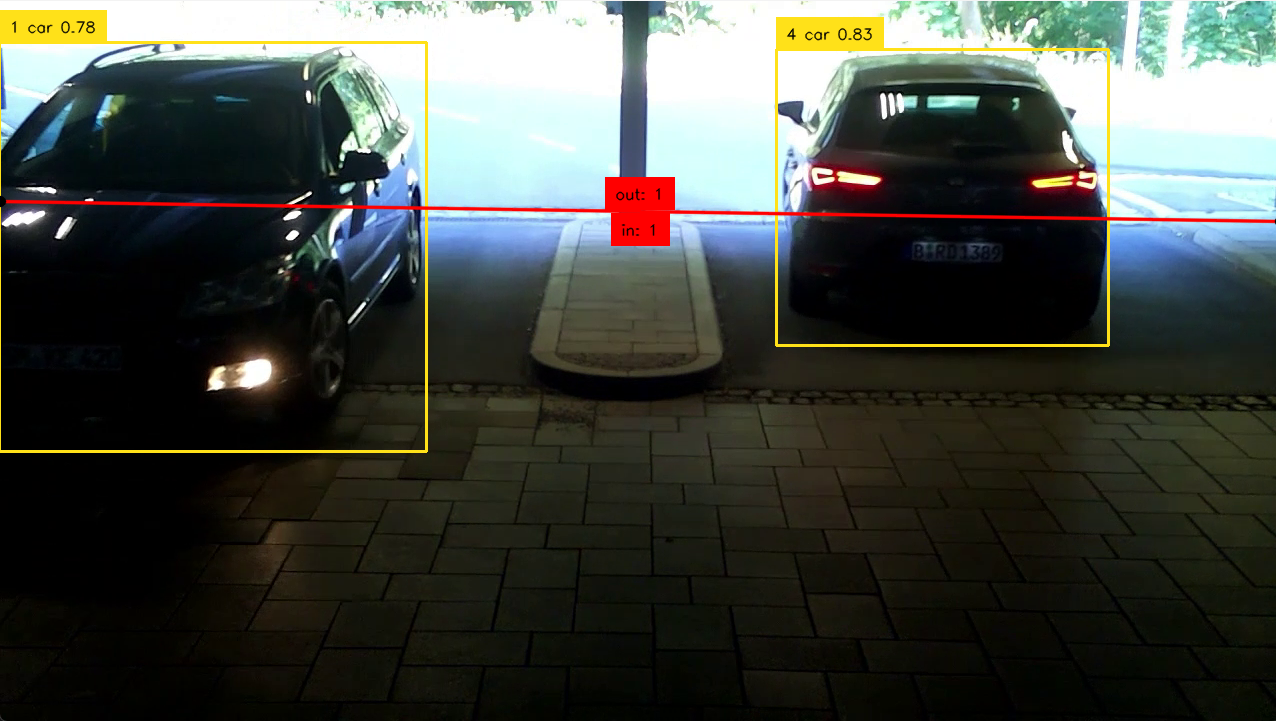
\includegraphics[width=\myImageWidth]{Bilder/Method3_Beispiel.png}
	\caption[Fahrzeugerkennung Variante 2 Beispiel]{Beispiel der Fahrzeugerkennung mit Variante 2 (Quelle: eigene Darstellung)}
	\label{fig:Variante2}
\end{figure}

Es wird YOLOv8 eingesetzt, um die Fahrzeuge in den einzelnen Frames des Videos zu erkennen.
Der Vorteil des Frameworks ist es, dass es Objekten IDs zuordnen kann.
Somit ist eine eindeutige Zuordnung eines Autos über mehrere Frames hinweg möglich.
Die Zuordnung einer ID zu einem konkreten Auto über eine gewisse Dauer geschieht über verschiedene Merkmale des Objektes, wie die Eckpunkte der Objekterkennung, die Geschwindigkeit des Autos oder die Veränderung der Zuverlässigkeitswerte des Algorithmus.
Die erkannten Fahrzeuge werden durch ihre Eckkoordinaten repräsentiert.
Der daraus errechnete Mittelpunkt gibt Aufschluss über die Position des Fahrzeuges.

Der Algorithmus nutzt die erfassten Zählerwerte, um die aktuelle Auslastung des Parkhauses an einen Server zu übertragen.
Dazu wird eine HTTP PUT-Request im JSON-Format verwendet, um die Zählerwerte an den Server zu senden und die Fahrzeugbewegungen zu protokollieren.
\selectlanguage{ngerman}
\subsection{Server}\label{ch:Umsetzung_Server}
% - Geschrieben in Go 
% - Input als HTTP Schnittstelle
%   - in Produktion: Verwendung von HTTPS
%       - dann Basic Auth kein Problem 
%       - jeder Sensor hat Username (site_id) und Passwort das (als Hash) manuell in die SQLite DB eingetragen werden muss
%       - sowieso Pushen, daher egal ob Publish via MQTT oder HTTP Request (PUT)
% - Output als HTTP und MQTT 
%   - Vorteil MQTT: Abonnieren statt Pullen
%   - MQTT: 
%       - Topic ist die site_id
%       - beim Verbinden wird letzter Stand geschickt (retain=true)
%       - Server ist Broker
%       - Clients dürfen nur subscriben, nicht publishen; jeder darf verbinden (keine Beschränkung auf IP-Adressen oder Anmeldung mit Passwort)
% - Anbindung an SQLite DB
%   - 2 Tabellen
%   - sites: Speicherung der Zugangsdaten
%   - counter: Speicherung der Zählerstände
% - ursprünglicher Eintrag (Maximale Anzahl der Autos (max_cars), Anzeigename des Parkplatzes (display_name), ID (site_id) und Passwort Hash (password_hash)) in DB muss manuell geschehen
%   - In finalem Produkt wäre ggf. zusätzliche Anwendung für Mitarbeiter notwendig

Der Server wurde in der Programmiersprache Go entwickelt und dient zur Verwaltung und als zentrale Stelle der Kommunikation für die Übermittlung der Zählerwerte von Sensor zum Endnutzer.

Zum Entgegennehmen der Werte vom Sensor wird die HTTP-Schnittstelle \lstinline|PUT /api/v1/c/{site_id}| zur Verfügung gestellt.
Die Daten werden für diese im HTTP Body in JSON übertragen.
Das vom Server erwartete JSON Objekt, welches nachfolgend beispielhaft dargestellt ist, enthält dabei aktuell lediglich das Attribut \lstinline|currentCars|, welches den aktuellen Zählerstand als Ganzzahl enthält.

\lstset{language=json, numbers=none}
\begin{center}
    \begin{mylisting}[hbox,enhanced,drop shadow]{Input JSON}
{
    "currentCars": 60
}
    \end{mylisting}
\end{center}

Damit diese HTTP-Request zum Ändern des Zählerstandes nicht von jedem ungeschützt verwendet werden kann, ist eine Authentifikation nötig.
Konkret besitzt hierzu jeder Sensor, der mit dem Server verbunden ist, einen eindeutigen Benutzernamen (\lstinline|site_id|) sowie ein Passwort.
Zur Authentifizierung mit dem Server wird hierzu die HTTP Basic Authentication genutzt, bei welcher Nutzername (\lstinline|site_id|) und Passwort im HTTP Header als Base64 String kodiert übertragen werden.
Auf komplexere Authentifizierungsverfahren, wie beispielsweise JSON Web Tokens (JWT) wurde verzichtet, da die gebotenen Vorteile, wie beispielsweise die Möglichkeit zum clientseitigen Ausloggen, das automatische Ablaufen des Tokens oder der Schutz vor Klau des Passworts durch Verwendung des Tokens, in diesem Anwendungsfall als API nicht benötigt werden.
Zu Entwicklungszwecken wurde bisher auf die Verwendung von einer verschlüsselten Datenübertragung mittels HTTPS verzichtet.
In einer Produktivumgebung sollte zwingend \mbox{HTTPS} verwendet werden, um eine geschützte Übertragung zu gewährleisten.
Besonders wichtig ist dies, weil ohne verschlüsselte Verbindung das Passwort abgefangen werden kann.

Als Ausgabeschnittstelle stellt der Server die Daten sowohl über HTTP als auch über MQTT bereit.
Mittels HTTP kann über die Schnittstelle \lstinline|GET /api/v1/c/{site_id}| das JSON Objekt, welches nachfolgend beispielhaft zu sehen ist, mit den Zählerinformationen abgerufen werden.
Der Vorteil von MQTT besteht darin, dass Clients Daten abonnieren können, anstatt sie aktiv abzurufen.
Der Server fungiert als MQTT-Broker und Clients können sich mit ihm verbinden, um Topics zu abonnieren und bei Änderungen dieser die Daten zu empfangen.
Die \lstinline|site_id| wird hierbei als Topic des MQTT-Protokolls verwendet.
Sobald vom Sensor, wie zuvor beschrieben, mittels HTTP der Zählerstand aktualisiert wird, publisht der Server diesen auf die entsprechende MQTT-Topic.
Beim Verbinden mit dem MQTT-Server wird der letzte bekannte Zustand an den Client gesendet, da das \lstinline|retain|-Flag auf \lstinline|true| gesetzt ist.
Somit sind direkt aktuelle Daten verfügbar, ohne dass zunächst eine Änderung durch den Sensor gemeldet werden muss.
Die Clients haben jedoch keine Berechtigung, Daten zu veröffentlichen (publishen).
Es gibt daher keine Beschränkungen für die MQTT-Verbindung aufgrund von IP-Adressen oder Anmeldungen mit Passwörtern.

\lstset{language=json, numbers=none}
\begin{center}
    \begin{mylisting}[hbox,enhanced,drop shadow]{Output JSON}
{
    "id": "HS_Coburg",
    "displayName": "Parkhaus Hochschule Coburg",
    "currentCars": 100,
    "maxCars": 530
}
    \end{mylisting}
\end{center}

Zur Speicherung der relevanten Informationen verwendet der Server eine SQLite-Datenbank mit zwei Tabellen.
Die erste Tabelle, \lstinline|counter|, speichert die aktuellen Zählerstände sowie gleichbleibende Daten der Sensoren, wie beispielsweise die maximale Anzahl der Autos, die im JSON der Ausgabeschnittstelle vorhanden sind.
Die zweite Tabelle, \lstinline|sites|, enthält die Zugangsdaten für die einzelnen Sensoren.
Das Passwort wird hierbei nur als Hash-Wert gespeichert.
Die Einträge zu Zugangsdaten und Details der Parkplätze müssen zuvor manuell in die Datenbank eingetragen werden.
Hierzu wäre es in einem finalen Produkt möglicherweise erforderlich, eine zusätzliche Anwendung für Mitarbeiter bereitzustellen.
Diese Anwendung könnte eine Benutzeroberfläche bieten, um neue Sensoren hinzuzufügen, ihre Zugangsdaten einzugeben und weitere Konfigurationen vorzunehmen.
Für den Rahmen des aktuellen Prototyps genügt die Oberfläche von Drittanbieter Datenbanksoftware, wie beispielsweise der \textit{DB Browser for SQLite}.

\selectlanguage{ngerman}
\subsection{App}\label{ch:Umsetzung_App}
% - Geschrieben mit Flutter und Dart
%   --> verschiedene Plattformen (Android, Windows, iOS, macOS, ...)
% - abonniert via MQTT die Topic (im Prototyp ist Topic hartkodiert; final Auswahl aus Liste, wenn allgemeine App)

Um die aktuelle Parkhausbelegung für den Nutzer darzustellen, wurde eine App entwickelt, die mithilfe von Flutter und Dart geschrieben wurde und daher verschiedene Plattformen, wie Android, Windows, iOS und macOS, bedient.
In Abbildung~\ref{fig:app} sind Screenshots der App dargestellt.

\begin{figure}[h]
	\centering
	\subfloat{
		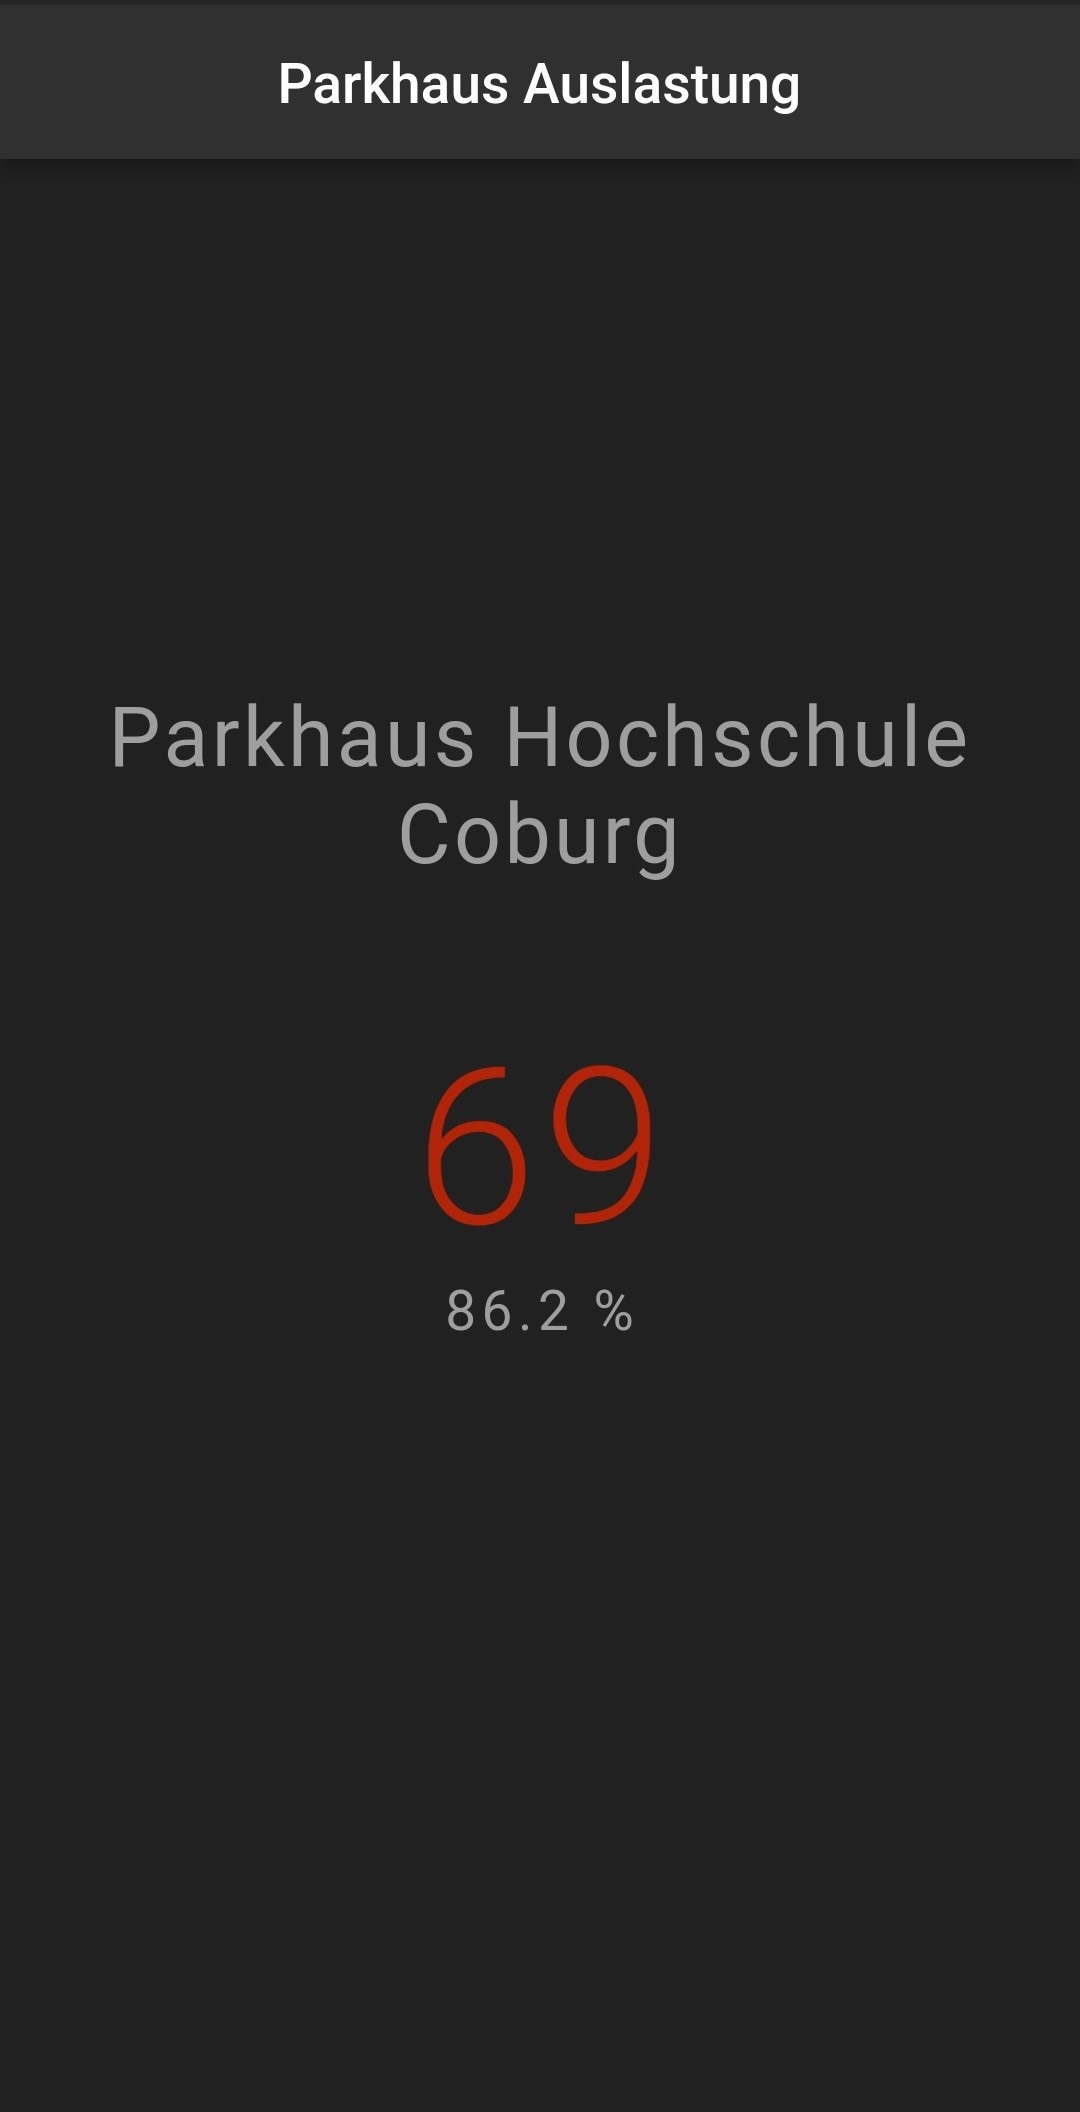
\includegraphics[width=0.3\myImageWidth]{Bilder/app_69.jpg}}
	\hfill
	\subfloat{
		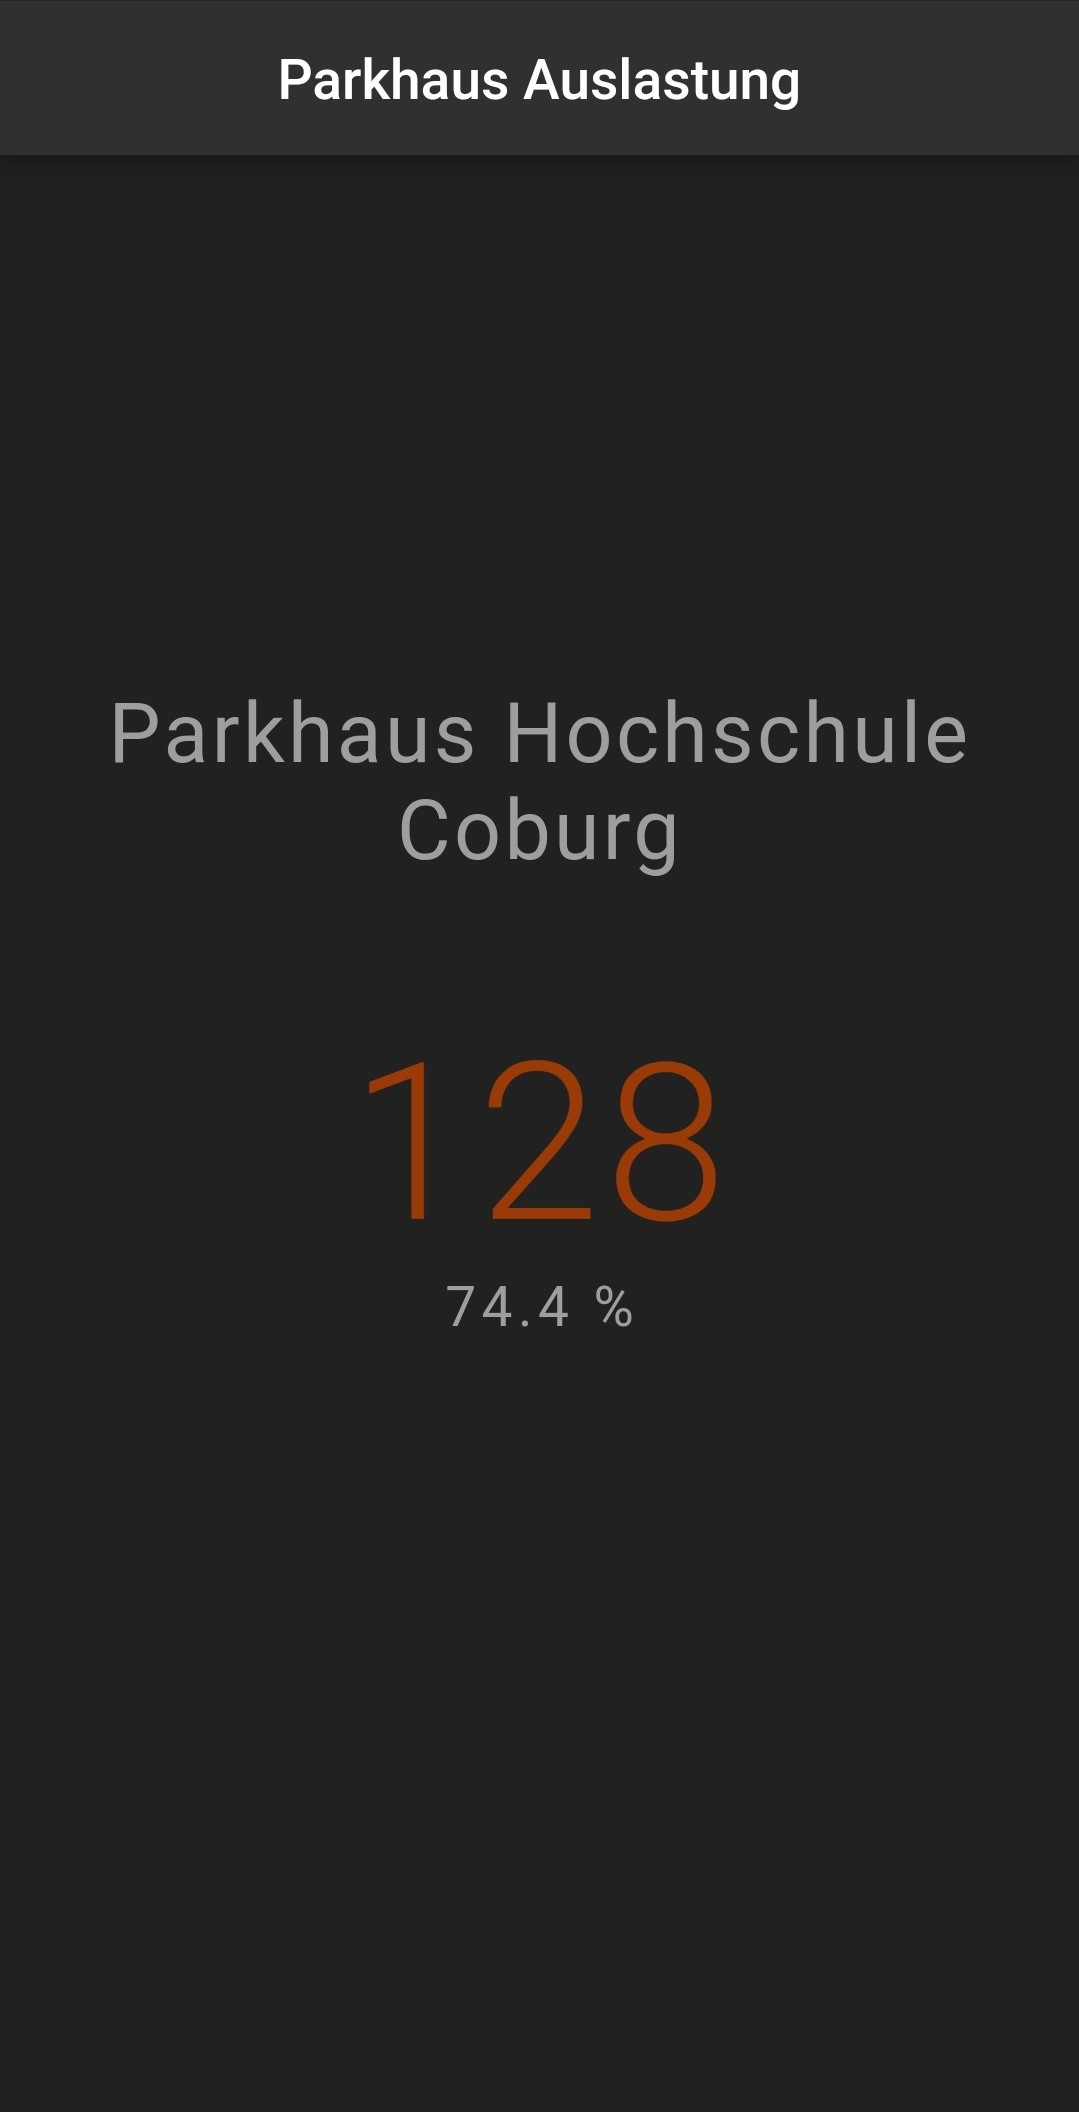
\includegraphics[width=0.3\myImageWidth]{Bilder/app_128.jpg}}
	\hfill
	\subfloat{
		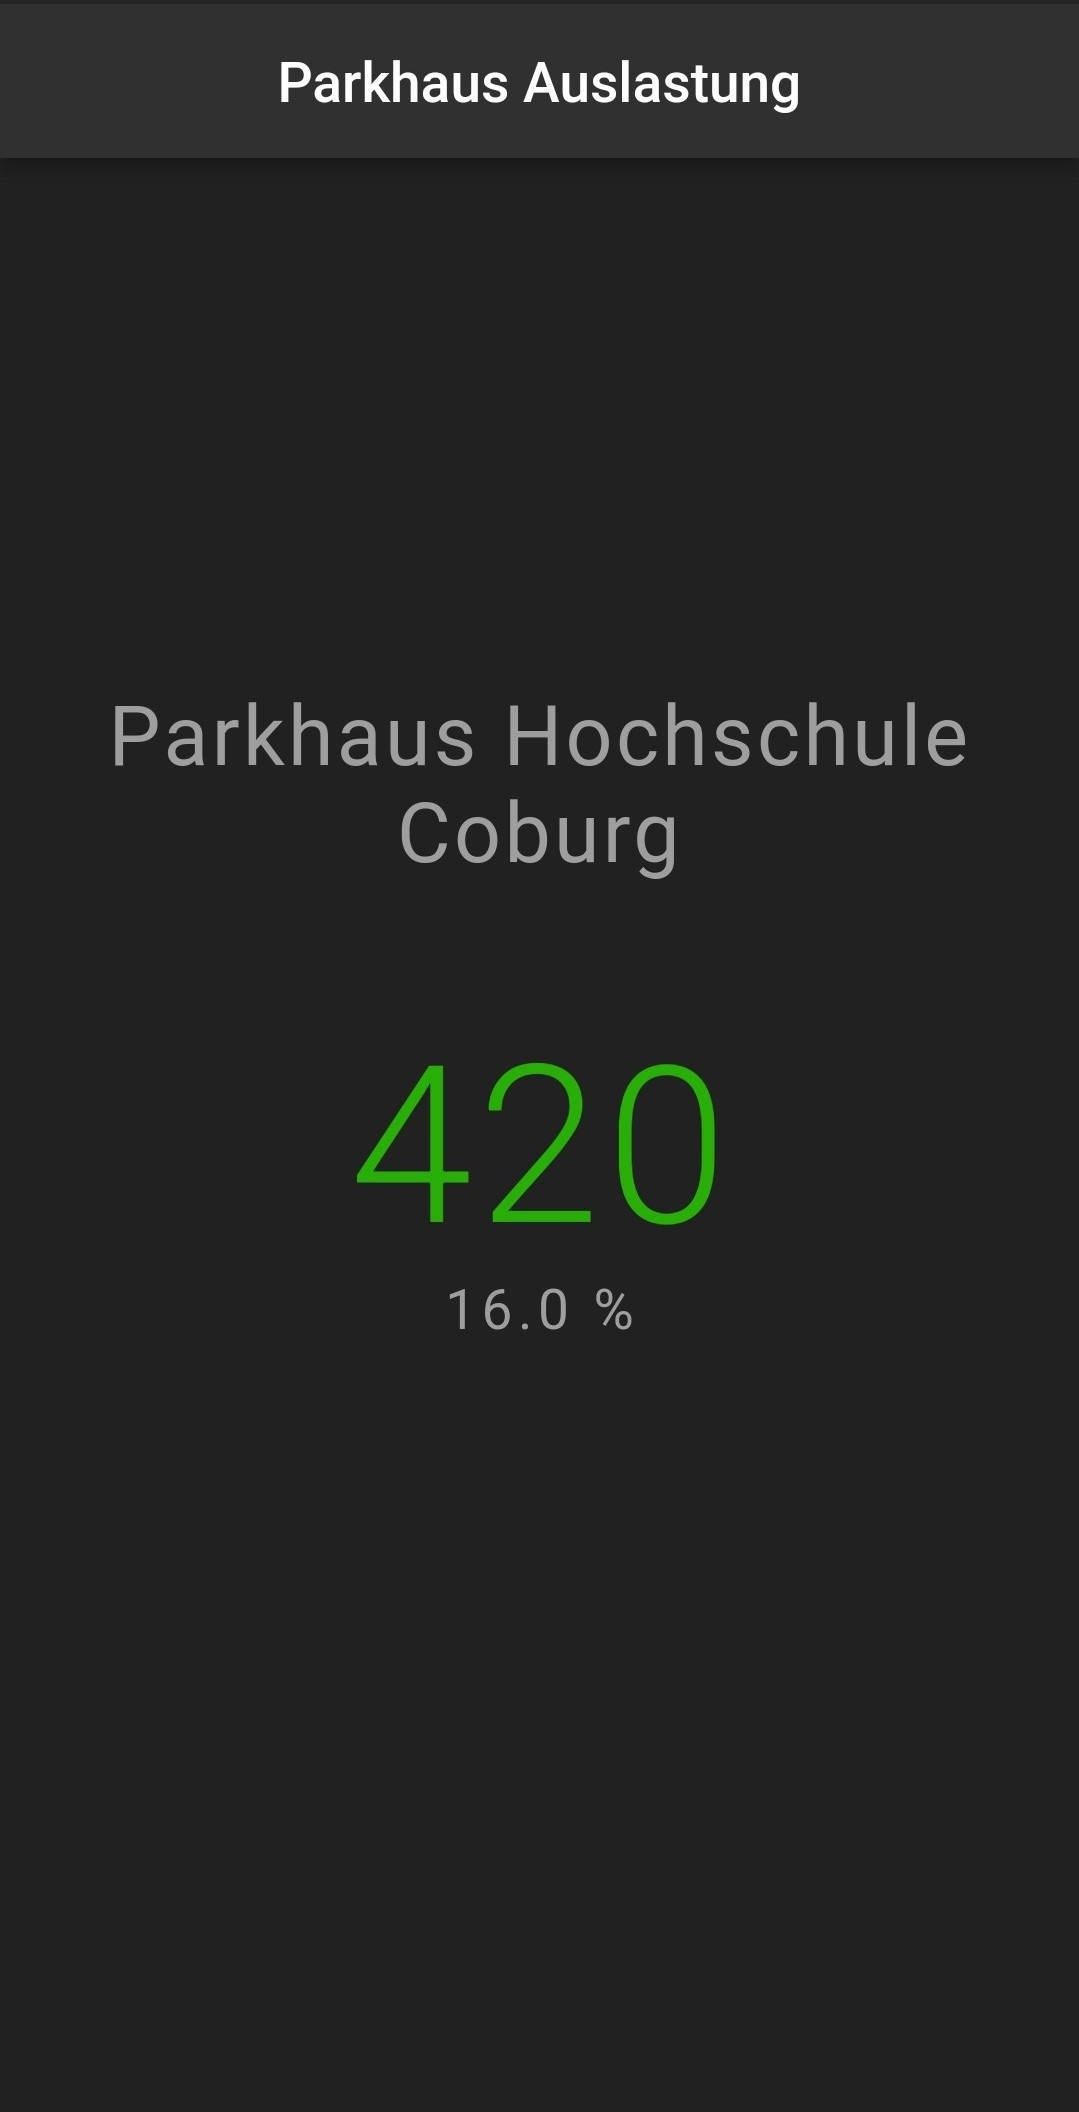
\includegraphics[width=0.3\myImageWidth]{Bilder/app_420.jpg}}
	\caption[Screenshots der App]{Screenshots der App (Quelle: eigene Darstellung)}\label{fig:app}
\end{figure}

Flutter und Dart stellen ein leistungsstarkes Framework und eine Programmiersprache dar, die von Google entwickelt wurden, um die Entwicklung plattformübergreifender Apps zu vereinfachen.
Flutter ermöglicht die Erstellung reaktiver Benutzeroberflächen, während Dart eine effiziente und objektorientierte Programmierung unterstützt.
Die Verwendung einer einzigen Codebasis für verschiedene Plattformen verbessert die Wartung und Skalierbarkeit der App erheblich.~\cite{awsWasIstFlutter}~\cite{dartDartOverview}

Wie bereits genannt, dient MQTT als leichtgewichtiges und zuverlässiges Kommunikationsprotokoll zum Empfangen der Nachrichten.
Die App abonniert die Topic des entsprechenden Parkplatzes beim Broker, um diese Informationen anzuzeigen.
Im aktuellen Prototypen ist die Topic hartkodiert.

